\chapter{Campaign and Analysis}
\label{campaign_and_analysis}
The Analysis of this campaign bases of the observation campaign of NGC4593 in 2016 by Edward M. Cackett \parencite{cackett2018accretion}. The observations took place between the 12th of July and the 6th of August with 26 successful observations out of 27 and was performed with the Hubble Space Telescope (HST) using the Space Telescope Imaging Spectrograph (STIS). The following section will cover important properties of NGC4593 and the 2016 campaign.

\section{NGC4593}
\label{NGC4593}

NGC 4593 is an active galactic nucleus (AGN), classified as a Seyfert 1 galaxy with a \mbox{(R)SB(rs)b} barred spiral morphology. 
It is located in the southern sky at RA = 12:39:39.44, DEC = $-05$°$ 20' 39.03''$ (J2000) and has a redshift of $z = 0.0083 \pm 0.0005$, corresponding to a distance of about $35.6$ Mpc \parencite{simbaNGC4593} based on the $\Lambda$CDM model. 
The galaxy exhibits a prominent large-scale bar and nuclear dust ring connected to dust lanes along the bar, which likely channel gas toward the central region \parencite{mulchaey1997structure}, as seen in figure \ref{fig:NGC4593}. 
The AGN shows strong broad emission lines in  H$\alpha$,  H$\beta$,  H$\gamma$, Ly$\alpha$, He\,\textsc{i}, and He\,\textsc{ii} \parencite{bentz2015agn}, indicating a well-developed broad-line region. 
Reverberation mapping of the broad H$\beta$ line yields a supermassive black hole mass of $M = \left(7.63 \pm 1.62\right) \times 10^6\,M_\odot$ \parencite{bentz2015agn}, with a corresponding broad-line region radius of only a few light-days \parencite{denney2006ngc4593}. 
Multi-wavelength monitoring has revealed strong variability from X-ray to optical bands, with interband time delays indicating a UV/optical-emitting accretion disk about three times larger than predicted by standard thin-disk theory and signatures of diffuse continuum emission from the BLR, particularly around the Balmer jump \parencite{cackett2018accretion}. 
ALMA observations further reveal a central molecular gas reservoir of $\sim 10^8\,M_\odot$ arranged in a one-armed spiral and a circumnuclear ring, as well as evidence for a mild molecular outflow on scales of a few hundred parsecs \parencite{garcia2019alma}, highlighting the interplay between bar-driven inflow and AGN feedback in this galaxy. 

\begin{figure}[!ht]
	\centering
	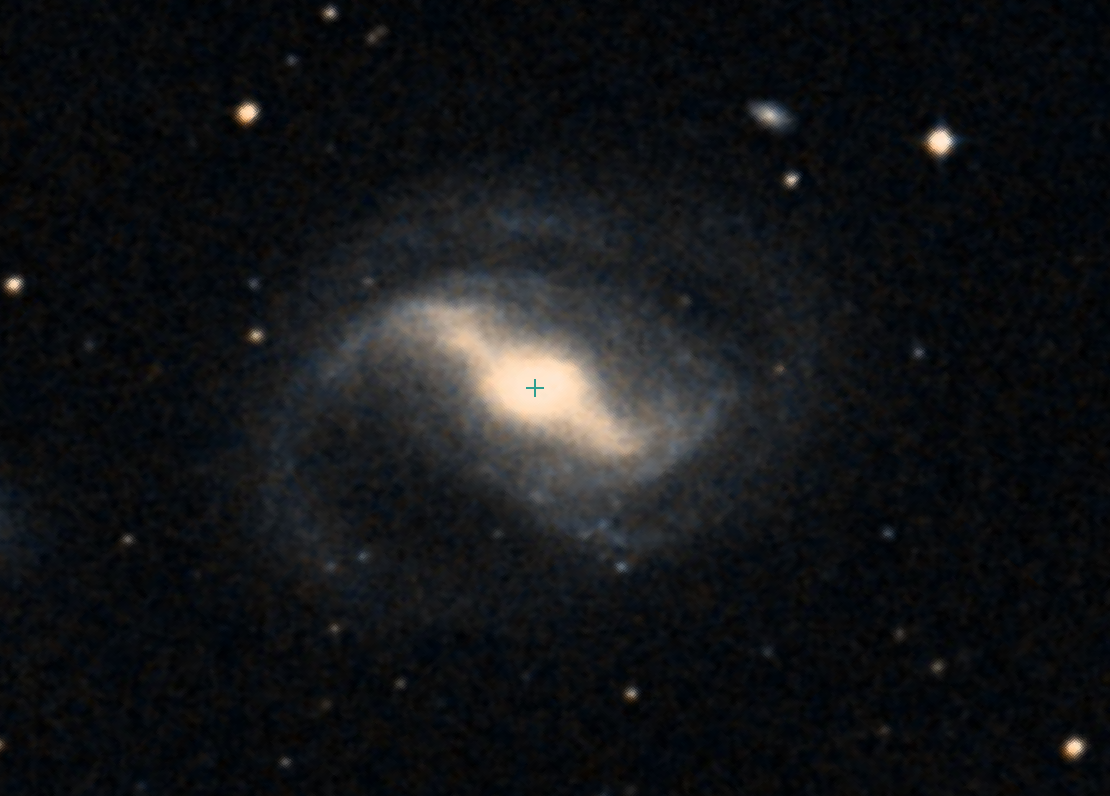
\includegraphics[width=0.5\textwidth]{pictures/Chapter3/NGC4593.PNG}
	\caption{A DSS image of NGC4593.}
	\label{fig:NGC4593}
\end{figure}

\section{2016 Campaign by E. M. Cackett}
\label{Campaign_Cackett}

E. M. Cackett's campaign was designed to study wavelength dependent continuum lags. Therefore, the STIS instrument on the Hubble Space Telescope was used with low-resolution gratings to measure a broad range of wavelengths. In each observation, spectra were taken using three different gratings: G140L, G430L, and G750L. These were used together with the $52'' \times 0.2''$ slit.\\
The characteristics of the STIS gratings used in this analysis are summarized in Table \ref{tab:stis_gratings}. After a standard pipeline-processing, a package was used to do a Charge Transfer Inefficiency correction with an algorithm based on \parencite{anderson2010empirical}. The few left rest of hot pixels got manually removed by interpolating the flux of neighbor pixels.\\


\begin{table}[h!]
	\centering
	\small
	\caption{Overview of STIS Grating Characteristics \parencite{stisgratings}}
	\label{tab:stis_gratings}
	\begin{tabular}{lcccc}
		\hline
		\textbf{Grating} & \textbf{Range [\AA]} & \textbf{Exp. Time [s]} & \textbf{Res. Power} & \textbf{Dispersion [\AA/pixel]} \\
		\hline
		G140L  & 1119--1715  & 1234 & $\sim 1000$         & 0.6 \\
		G430L  & 2888--5697  & 298  & $\sim 500 - 1000$    & 2.73 \\
		G750L  & 5245--10233 & 288  & $\sim 500 - 1000$    & 4.92 \\
		\hline
	\end{tabular}
\end{table}

\newpage


\section{Intercalibration and Determination of AVG- and RMS-Spectrum} 

To perform a reverberation mapping analysis it is essential to have multiple observations of the object to analyze its variability. In case of the 2016 campaign of NGC 4593, 26 of the 27 observations are usable. The epochs were downloaded from the ... archive and the faulty observation removed for the further analysis. The top panel of figure \ref{fig:comparison_spectra} shows parts of the optical spectral range of those epochs.\\
For the further analysis an average spectrum AVG gets obtained by averaging over all those epochs. In the best case this results in a signal-to-noise ratio in which it is possible to identify spectral features of NGC 4593s spectrum. Furthermore it is essential to identify variability between the epochs, which can be optained with the root-mean-spuare (RMS) spectrum. It is calculated as the standard deviation of the flux at each wavelength across all epochs:

\begin{equation}
	F_{\mathrm{RMS}}\left(\lambda\right) = \sqrt[]{\frac{1}{N-1}\sum_{N}^{i=1}\left(F_i\left(\lambda\right)- \bar{F}{\left(\lambda\right)}\right)^2}
\end{equation}

with the mean spectrum at $\lambda$:

\begin{equation}
	\bar{F} = \frac{1}{N} \sum_{N}^{i=1} F_i\left(\lambda\right)
\end{equation}
Constant features, such as narrow emission lines should be disappearing from the spectrum while Variable features, like the broad emission lines become strongly enhanced.\\
In the top panel of figure \ref{fig:comparison_spectra_avg_rms} the results of the AVG and RMS spectrum of the original data can be found. However the RMS spectrum shows still variation for not variating lines, especially for the forbidden lines at about $5000 \AA$.








\begin{figure}[!ht]
	\centering
	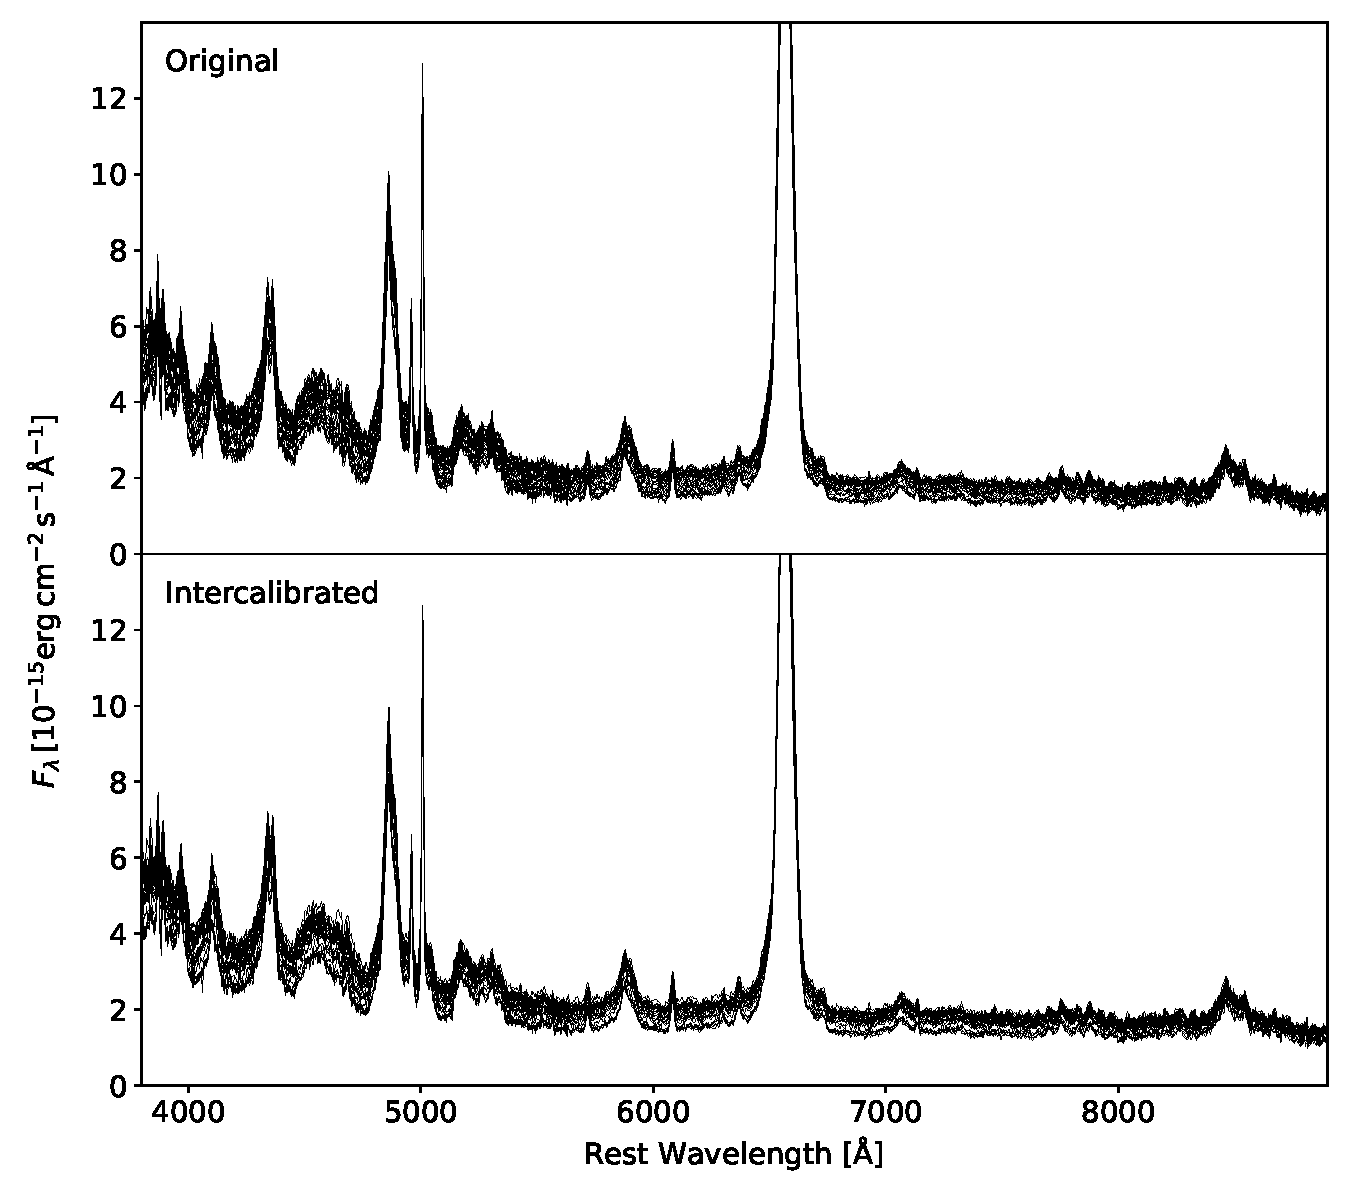
\includegraphics[width=\textwidth]{pictures/Chapter3/comparison_spectra}
	\caption{Comparison of the optical spectral range of the original spectra and the [O \textsc{iii}] $\lambda5007$ intercalibrated spectra from the 2016 campaign of NGC 4593.}
	\label{fig:comparison_spectra}
\end{figure}

\begin{figure}[!ht]
	\centering
	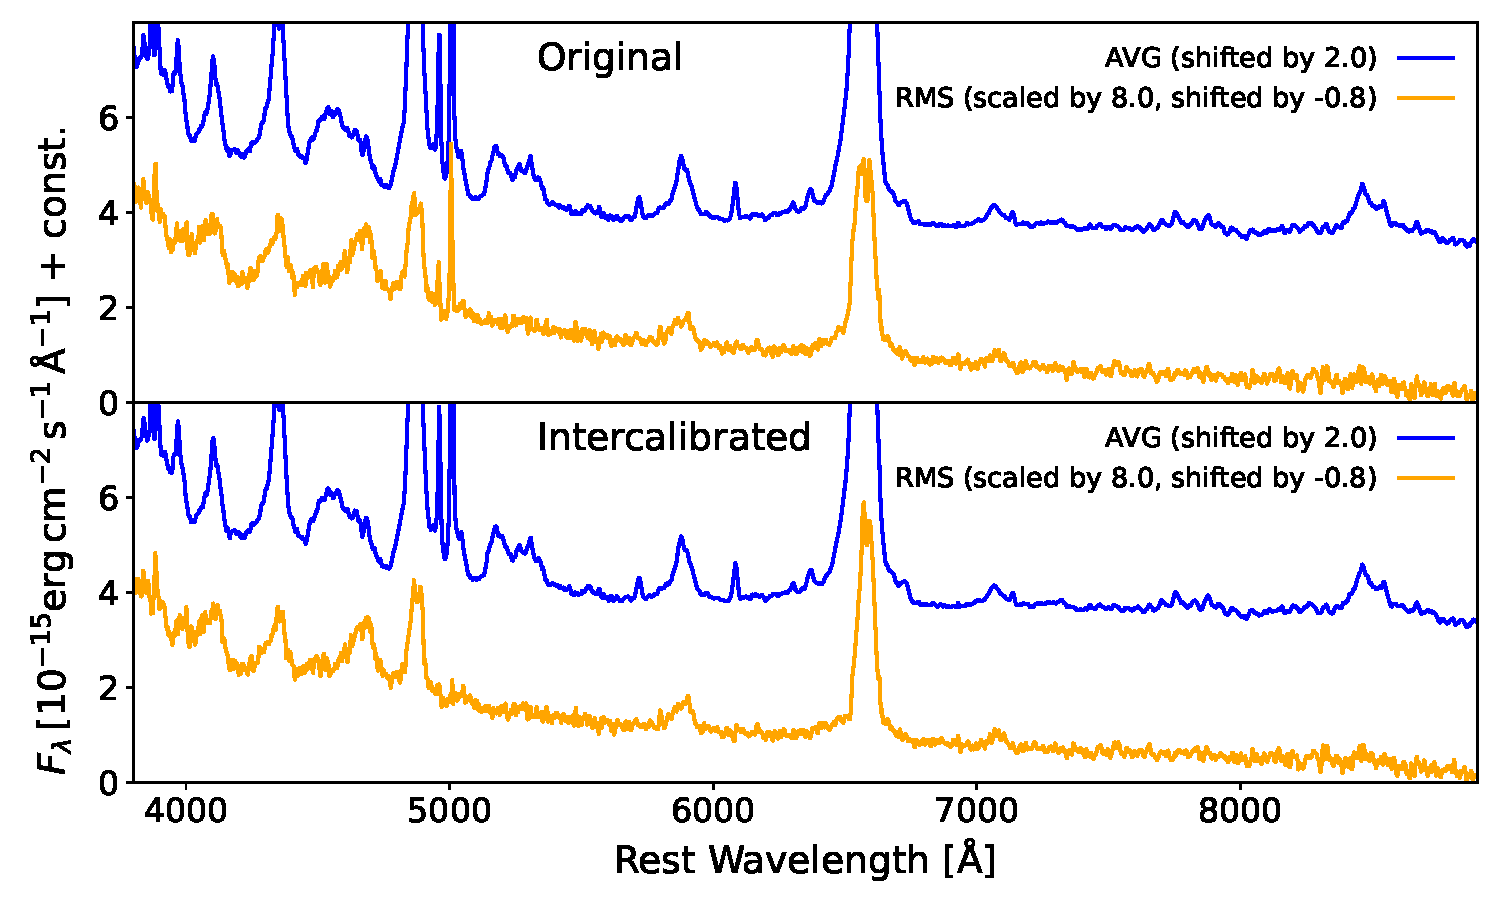
\includegraphics[width=\textwidth]{pictures/Chapter3/comparison_avg_rms}
	\caption{Comparison of the optical spectral range of the avg and rms spectra from the original data and the [O \textsc{iii}] $\lambda5007$ intercalibrated data from the 2016 campaign of NGC 4593.}
	\label{fig:comparison_spectra_avg_rms}
\end{figure}

\begin{figure}[!htbp]
	\centering
	\makebox[\textwidth][c]{%
		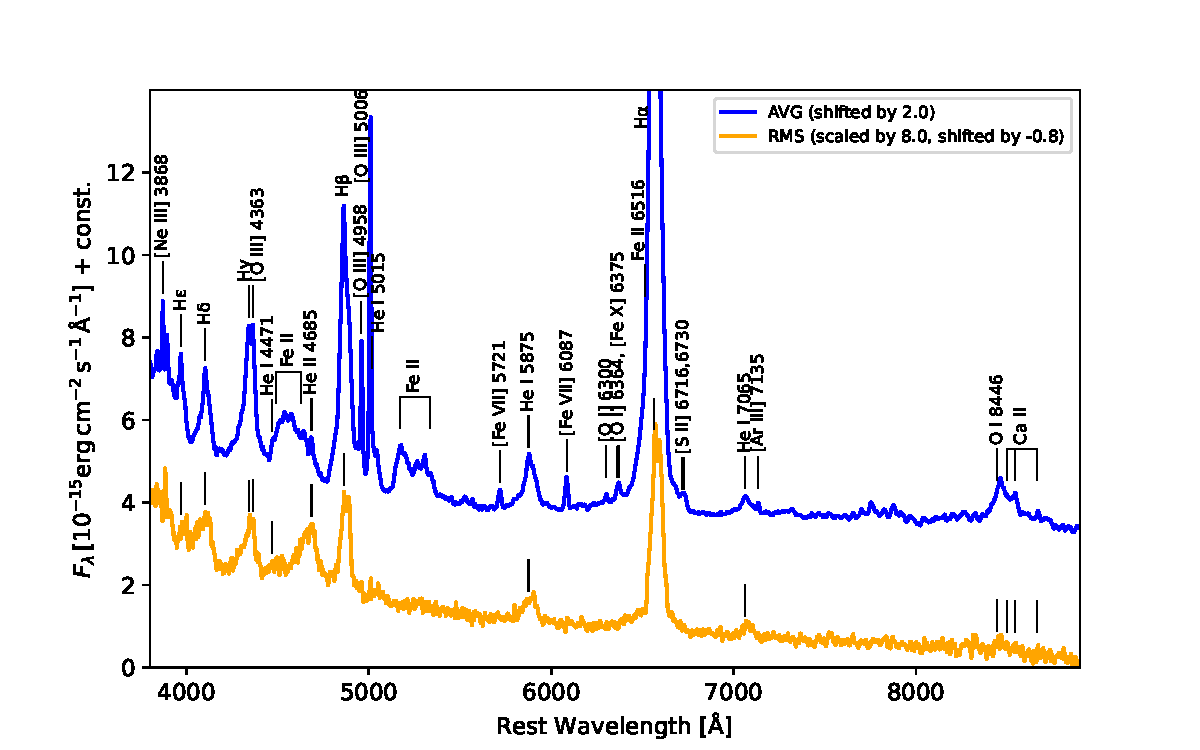
\includegraphics[width=1.2\textwidth]{pictures/Chapter3/avg_rms_spec.pdf}}
	\caption{AVG RMS spectrum}
	\label{fig:AVG_RMS_SPECTRUM}
\end{figure}
